\section{Database design description}
{\it Note the difference between 'main user' and 'user'. Main user refers to the user who owns the local database. 'User' or 'other user' refers to other users, usually the relations of the main user.}
\subsection{user table} 
This table stores user details, which includes the main user's own details and its relations. As the user makes a new relation with another user, its details will be stored in this table. Every user has their own public key which uniquely identifies their accounts which also be stored in this table.

\subsection{user, is\_in\_category, category table}
With the category table, the user can create new categories to group his relations. As it is possible for many users to belong in many categories, the {\it is\_in\_category} table is needed to identify which set of users belong in the categories.

\subsection{user, is\_invited, events table}
These tables suggest that users can create events. One particular feature regarding these tables that on the {\it is\_invited table}, where the user (the main one) can invite anyone individually from the relations list or as a group from the category list. However, there will be no tuples added under this table when another user posts the event. Reason being is that the main user is not allowed to see who the list of other users invited in the event which was not created by the main user. 

When the main user creates an event, he invites other people, either from the user table or from the category table or both. Once the invitation is sent out to those users, the users can either accept or reject the invitation. Using the {\it decision} attribute from the {\it is\_invited} table, if decision has not been made, it will be NULL. If user accepts the invitation, it will be 1 for true. If rejected, it will be 0 for false. 

\subsection{user, allowed\_to, wall\_post table}
When users create post, its data will be inserted into the {\it wall\_post} table. The attribute {\it from} refers to the user who has created the post, whilst the attribute {\it to} refers to the user who is referred or mentioned in this post. The main user can also choose a allow a set of his relations to view his post. Using the {\it allowed\_to} table, similar as the {\it is\_invited} table, the main user can select his relations either individually or through categories or both. If the post is created by another user, no tuples will be inserted into the {\it allowed\_to} table.

\subsection{user, has\_like, wall\_post table}
Users can like any posts that appears in his main wall or personal wall. When a post is liked, a new tuple is created in the has\_like table to indentify who liked the post, which post is liked, and the time the post is liked. These likes are counted and displayed in the GUI showing how many users have liked this post.

\subsection{user, has\_like, has\_comment table}
Other than liking posts, users can like individual comments as well. Same feature as liking the post by this time, data is inserted into the attribute {\it comment\_id} from the {\it has\_like} table to show which particular comment has been liked by this user.

\subsection{user, has\_comment, wall\_post table}
Users can comment on posts. When post is commented on, a new tuple will be added into the {\it has\_comment} table on information like the content of the comment, which post has been commented on, who commented on the post, and the time of comment.

\subsection{user, has\_comment table}
Users can also comment on comments itself. This will create and indentation on the GUI to suggest that the parent comment has a child comment. When a comment is commented upon, the attribute {\it comment\_comment\_id} will insert the parent comment\_id which shows the relation of two comments, one parent and the other being the child.

\subsection{user, is\_in\_message, private\_message table}
Another functionality found in Turtlenet is the user is able to send private messages to users. When a private message is created by the main user, a new tuple is added into the {\it private\_message} table. The user then has the option to add other user(s) into the conversation. When done so, a tuple or tuples, depending on the number of users he has added onto the conversation, are added into the {\it is\_in\_message} table. This inserts the information such as the time of when the user has been added into the conversation, the user's ID and message ID. The {\it private\_message} table on the other hand stores data such as the content of the message and the time for which this whole conversation was created. 

\subsection{message\_claim table}
When the main user has not required any public key from the other user he is intended to add, the details will be entered onto this table until which a pubic key is retrieved. When retrieved, this information found in this table will be deleted and transferred into the {\it user} table along with other information that comes with it.

\subsection{key\_revoke table}
In times when malicious activity might have been conducted, the users of Turtlenet is able to revoke their relations signature key. A signature suggests that this post is written by this person in particular, so when it is revoked, whatever that has been posted with this signature is considered false. This will inform the user not to trust any information that has been posted with this signature in particular. 

\subsection{login\_logout\_log table}
This table simply tracks the login and logout activities of the main user. When a user logs in and out, a new tuple will be inserted into this table.

\clearpage

\section{Table layout of the database}
NB: Public keys are 217 characters long, all id's are auto-incremented.

\begin{table}[!ht]
\caption{user}
\centering
\begin{tabular}{c c c}
\hline\hline
Name               & Datatype    & Key \\
\hline
user\_id           & INT          & PK \\  % 64-bit has key public key
username           & VARCHAR(25)  &    \\
name               & VARCHAR(30)  &    \\
birthday           & DATE         &    \\
sex                & VARCHAR(1)   &    \\
email              & VARCHAR(30)  &    \\
public\_key        & VARCHAR(600)   & PK \\
\hline
\end{tabular}
\label{table:nonlin}
\end{table}

\begin{table}[!ht]
\caption{is\_in\_category}
\centering
\begin{tabular}{c c c}
\hline\hline
Name               & Datatype    & Key \\
\hline
is\_in\_id         & INT     & PK   \\
category\_id       & INT     & FK   \\
user\_id           & INT     & FK   \\
\hline
\end{tabular}
\label{table:nonlin}
\end{table}

\begin{table}[!ht]
\caption{category}
\centering
\begin{tabular}{c c c}
\hline\hline
Name               & Datatype    & Key \\
\hline
category\_id       & INT         & PK  \\
name               & VARCHAR(30) &     \\
\hline
\end{tabular}
\label{table:nonlin}
\end{table}


\begin{table}[!ht]
\caption{private\_message}
\centering
\begin{tabular}{c c c}
\hline\hline
Name               & Datatype    & Key \\
\hline
message\_id        & INT         & PK  \\
from               & INT         &     \\
content            & VARCHAR(50) &     \\
time               & DATE        &     \\
\hline
\end{tabular}
\label{table:nonlin}
\end{table}

\begin{table}[!ht]
\caption{is\_in\_message}
\centering
\begin{tabular}{c c c}
\hline\hline
Name               & Datatype        & Key \\
\hline
is\_in\_id         & INT             & PK  \\
time               & DATETIME        &     \\
message\_id        & INT             & FK  \\
user\_id           & INT             & FK  \\
\hline
\end{tabular}
\label{table:nonlin}
\end{table}

\begin{table}[!ht]
\caption{wall\_post}
\centering
\begin{tabular}{c c c}
\hline\hline
Name                    & Datatype    & Key \\
\hline
wall\_id                & INT         & PK  \\
from                    & INT         & FK  \\
to                      & INT         & FK  \\
content                 & VARCHAR(50) &     \\
time                    & DATETIME    &     \\
\hline
\end{tabular}
\label{table:nonlin}
\end{table}

\begin{table}[!ht]
\caption{allowed\_to}
\centering
\begin{tabular}{c c c}
\hline\hline
Name                    & Datatype    & Key \\
\hline
allowed\_to\_id         & INT         & PK  \\
user\_id                & INT         & FK  \\
category\_id            & INT         & FK  \\
post\_id                & INT         & FK  \\
\hline
\end{tabular}
\label{table:nonlin}
\end{table}

\begin{table}[!ht]
\caption{has\_comment}
\centering
\begin{tabular}{c c c}
\hline\hline
Name                 & Datatype     & Key \\
\hline
comment\_id          & INT     & PK  \\
comment\_content     & VARCHAR(50)  &     \\
post\_id             & INT     & FK  \\
user\_id             & VARCHAR(50)  & FK  \\
comment\_comment\_id & INT     & FK   \\
time                 & DATETIME     &     \\
\hline
\end{tabular}
\label{table:nonlin}
\end{table}

\begin{table}[!ht]
\caption{has\_like}
\centering
\begin{tabular}{c c c}
\hline\hline
Name               & Datatype    & Key \\
\hline
like\_id           & INT          & PK  \\
post\_id           & INT          & FK  \\
user\_id           & INT          & FK  \\
comment\_id        & INT          & FK  \\
time               & DATETIME     &     \\
\hline
\end{tabular}
\label{table:nonlin}
\end{table}

\begin{table}[!ht]
\caption{events}
\centering
\begin{tabular}{c c c}
\hline\hline
Name                    & Datatype    & Key \\
\hline
event\_id               & INT          & PK  \\
title                   & VARCHAR(10)  &     \\
content                 & VARCHAR(40)  &     \\
time                    & DATETIME     & \\
start\_date             & DATETIME     & \\
end\_date               & DATETIME     & \\
from                    & INT          & FK  \\
\hline
\end{tabular}
\label{table:nonlin}
\end{table}

\begin{table}[!ht]
\caption{is\_invited}
\centering
\begin{tabular}{c c c}
\hline\hline
Name                    & Datatype    & Key \\
\hline
is\_invited\_id         & INT         & PK  \\
user\_id                & INT         & FK  \\
is\_in\_category\_id    & INT         & FK  \\
event\_id               & INT         & FK  \\
decision                & BIT         &     \\
\hline
\end{tabular}
\label{table:nonlin}
\end{table}

\begin{table}[!ht]
\caption{login\_logout\_log}
\centering
\begin{tabular}{c c c}
\hline\hline
Name               & Datatype    & Key \\
\hline
log\_id            & INT         & PK  \\
login\_time        & DATETIME    &     \\
logout\_time       & DATETIME    &     \\
\hline
\end{tabular}
\label{table:nonlin}
\end{table}

\begin{table}[!ht]
\caption{key\_revoke}
\centering
\begin{tabular}{c c c}
\hline\hline
Name               & Datatype    & Key \\
\hline
revoke\_id         & INT          & PK  \\
signature          & VARCHAR(45)  &     \\
time               & DATETIME     &     \\
\hline
\end{tabular}
\label{table:nonlin}
\end{table}

\begin{table}[!ht]
\caption{message\_claim}
\centering
\begin{tabular}{c c c}
\hline\hline
Name               & Datatype    & Key \\
\hline
username           & VARCHAR(25) & PK  \\
signature          & VARCHAR(45) &     \\
\hline
\end{tabular}
\label{table:nonlin}
\end{table}

\clearpage

\begin{landscape}
\begin{figure}[h]
    
    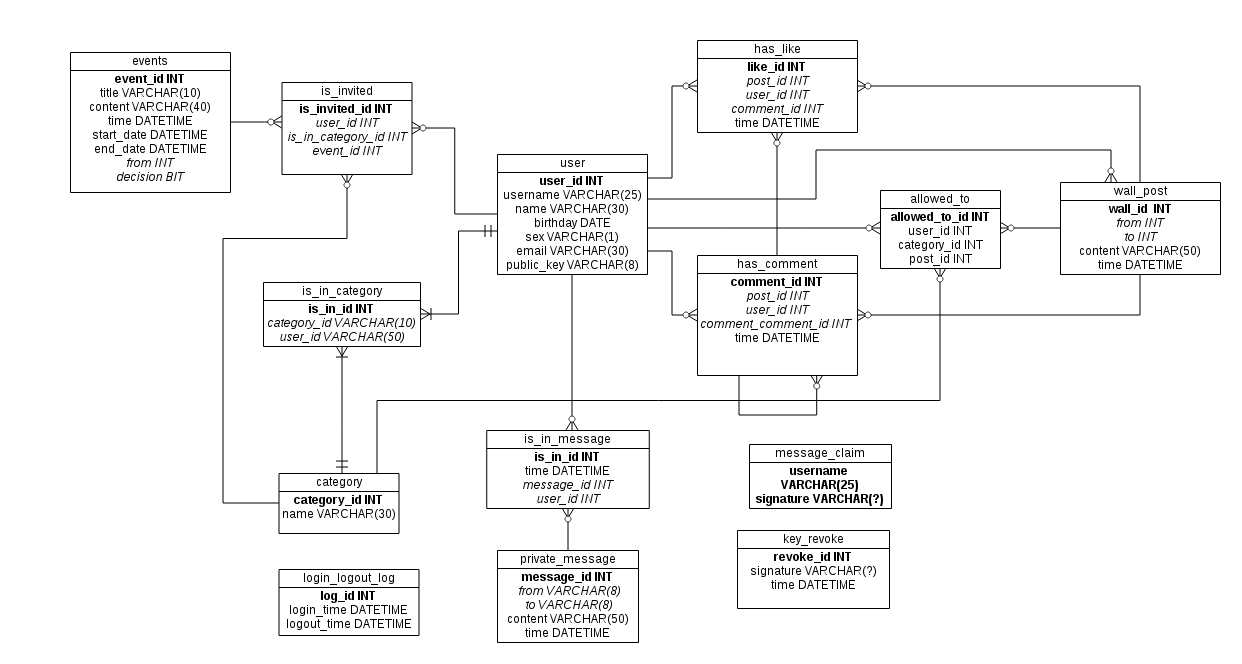
\includegraphics[width=1.4\textwidth]{images/design/project_er_diagram.png}
    \caption{Database Entity Relationship diagram}
    \label{fig:db_er_diag}
\end{figure}
\end{landscape}